\subsection{Video-Produktion}
Nach zahlreichen Ideensammlungen für die Erarbeitung eines Intros führte die gewünschte Stilrichtung stark in Richtung einer comichaften Animation, da sich das Projekt visuell hauptsächlich aus dieser Komponente zusammensetzt. Nach Recherchen für eine passende Entwicklungssoftware wurde das Programm AfterEffects von Adobe, aufgrund seiner hohen Professionalität und der vielen frei zugänglichen Tutorials im Internet, ausgewählt.

\subsubsection{Einarbeitung in After Effects}
Zunächst einmal erfolgte eine intensive Einarbeitungsphase mit dem Programm „After Effects“. Dabei waren sehr gute Youtube Tutorials eine große Unterstützung. 
Das Resultat von dem ersten Testvideo schaut wie folgt aus: 
\begin{figure}[h]
\centering
 \subfloat[Screenshot: After Effects 1]{{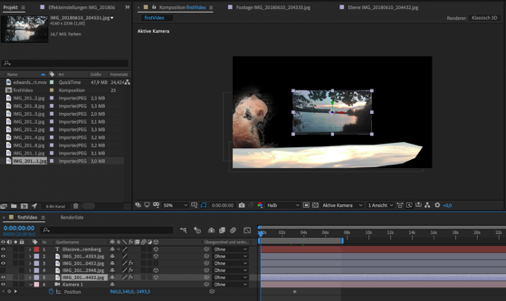
\includegraphics[width=5cm]{../img/screenshot_aftereffects_1.PNG} }}
\qquad
 \subfloat[Screenshot: After Effects 2]{{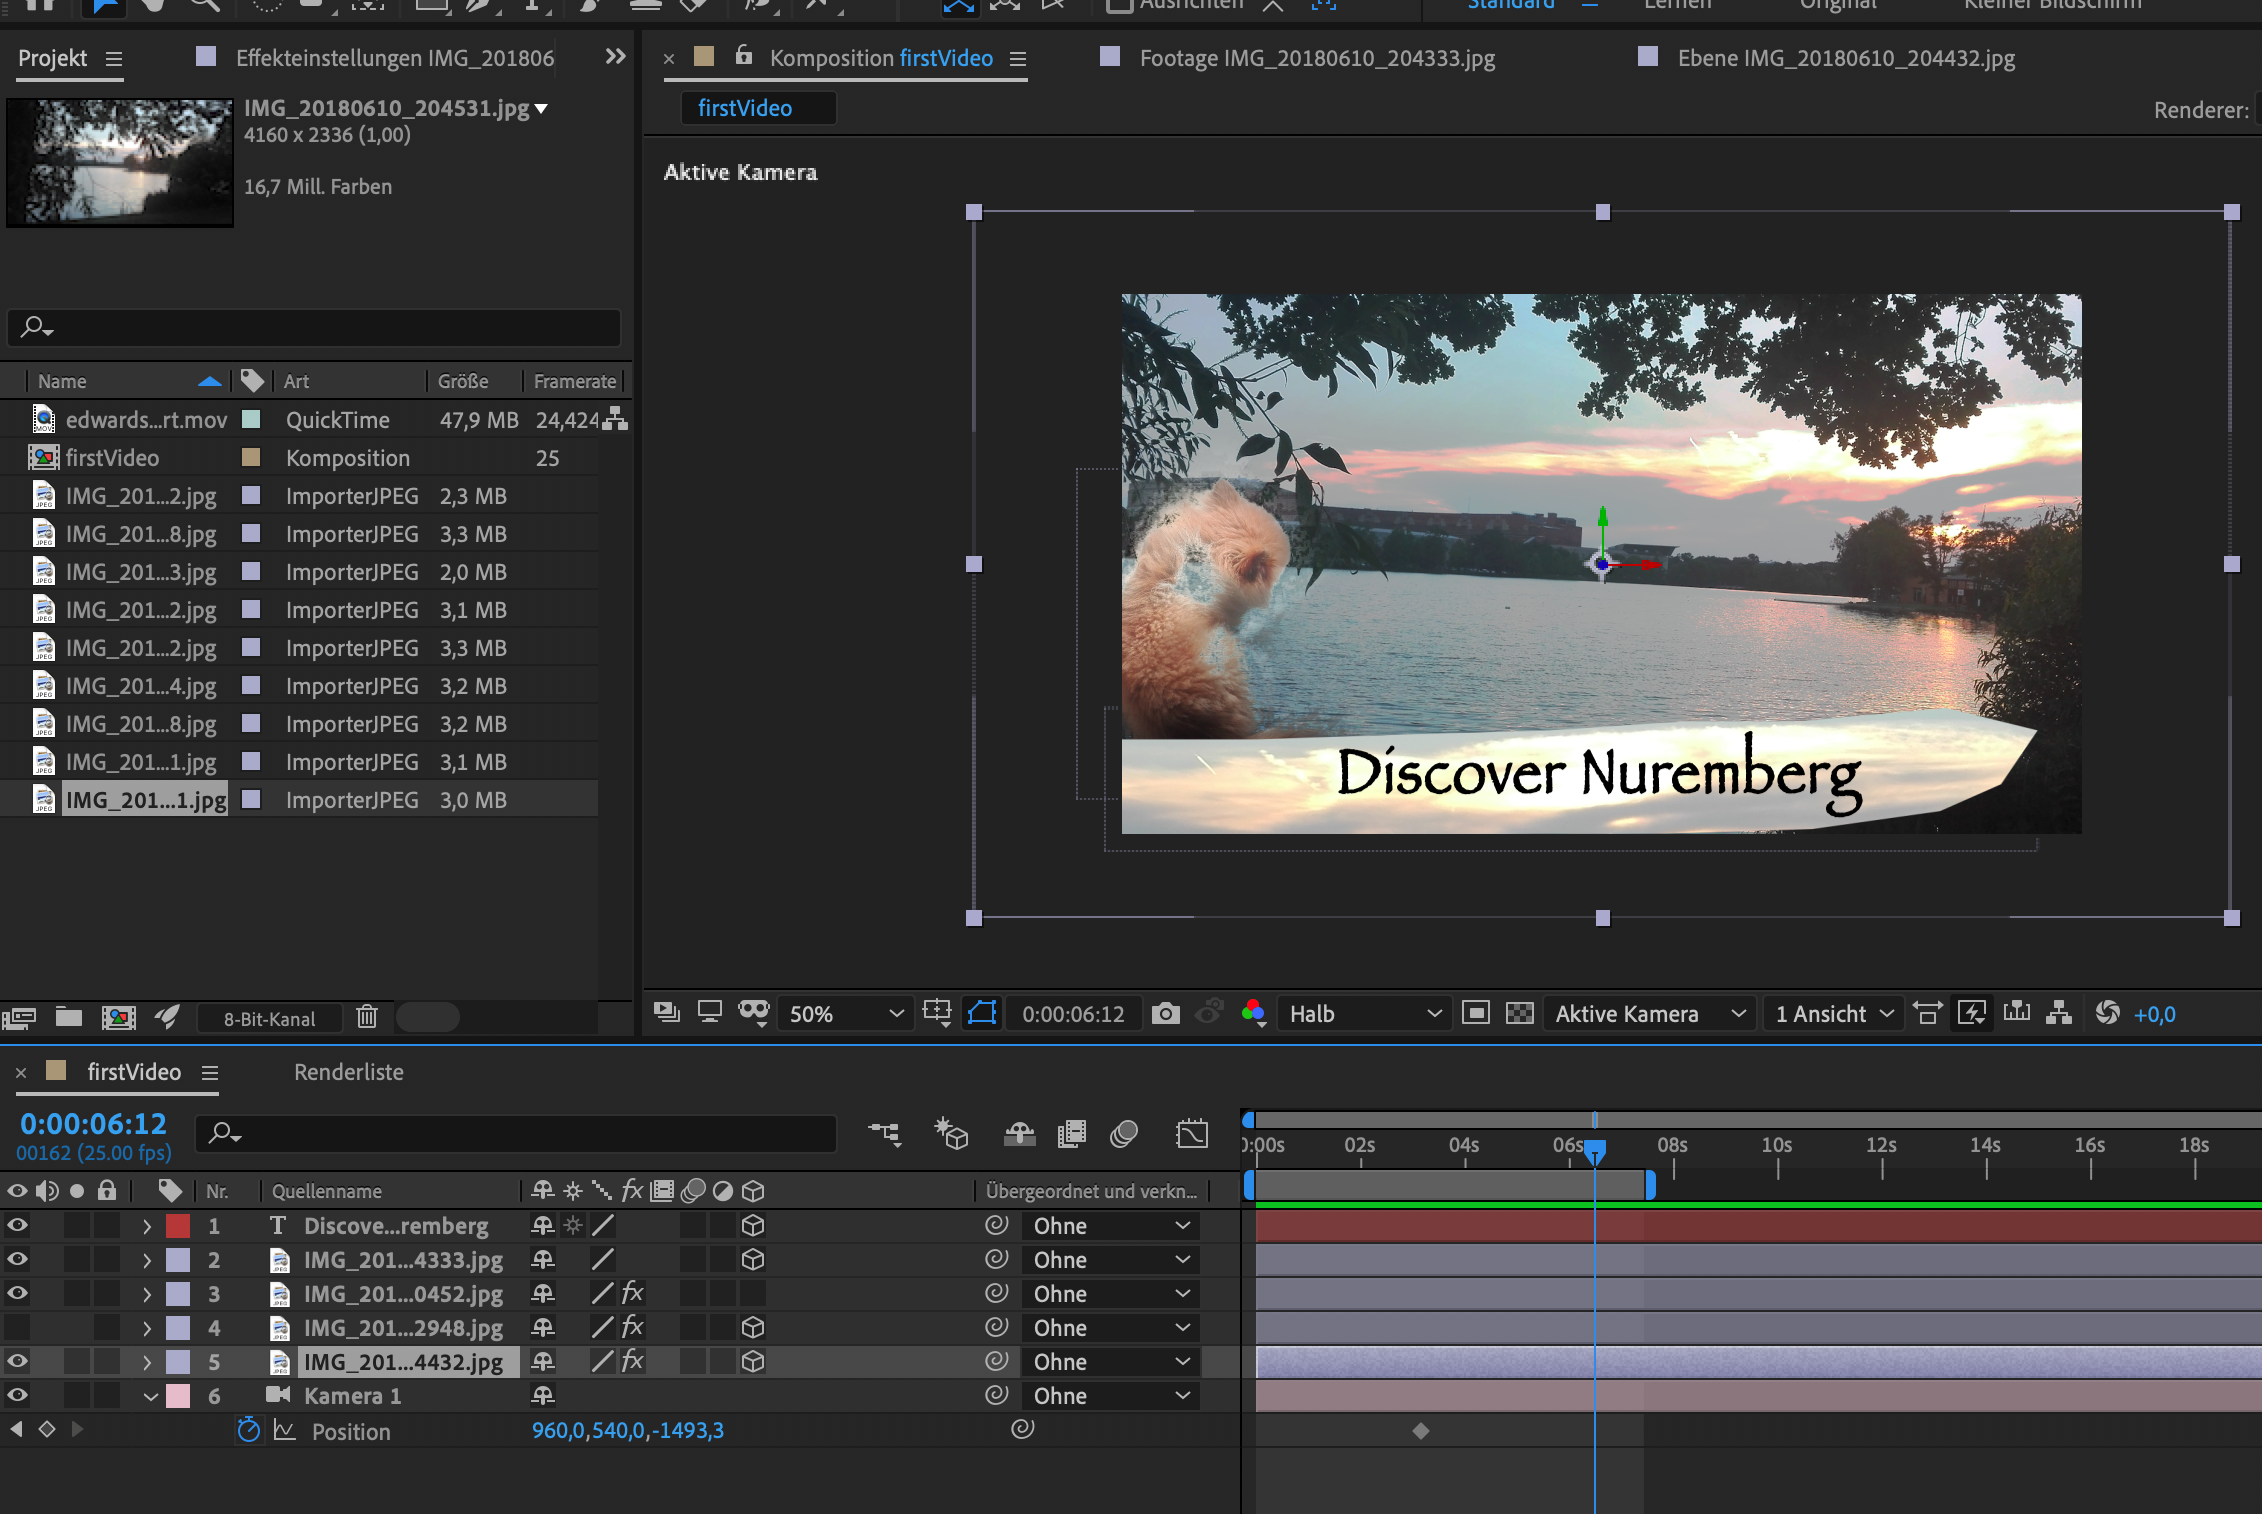
\includegraphics[width=5cm]{../img/screenshot_aftereffects_2.PNG} }}
\caption{Screenshots After Effects}%
 \label{fig:Screenshots After Effect}%
\end{figure}
Hierbei wurden Bilder freigestellt, ein Bild und der Titel animiert.  

\subsubsection{Animation des Logos}
Das Video endet, wie in vielen bekannten Videos, mit unserem Logo. Hierfür musste das Edwards Biotope Logo animiert werden. 
Zunächst einmal wurde die Grafik (links) von dem Text (rechts) separiert. Die Absicht war es, zuerst das Symbol animiert einzublenden. Im Anschluss taucht der Name „Edwards Biotope“ auf. Dieser Text wurde ebenso animiert. Zum Schluss werden beide Teile wieder zusammengefügt. Die Bildreihenfolge Abbildung \ref{fig:Screenshots Animations 1} stellt diese Logo Animation dar. 
\begin{figure}[h]
\centering
 \subfloat[Screenshot: Animation 1]{{
\includegraphics[width=2cm]{../img/logo_animation/1/screenshot_logo_1.PNG} }}
\qquad
 \subfloat[Screenshot: Animation 2]{{
\includegraphics[width=2cm]{../img/logo_animation/1/screenshot_logo_2.PNG} }}
\qquad
 \subfloat[Screenshot: Animation 3]{{
\includegraphics[width=2cm]{../img/logo_animation/1/screenshot_logo_3.PNG} }}
\qquad
 \subfloat[Screenshot: Animation 4]{{
\includegraphics[width=2cm]{../img/logo_animation/1/screenshot_logo_4.PNG} }}
\caption{Screenshots Animations 1}%
 \label{fig:Screenshots Animations 1}%
\end{figure}

Allerdings war das nicht sehr überzeugend. Daher wurde weiterhin experimentiert. So wurde das Logo mit dem Spielnamen nicht mehr separiert animiert, sondern von Anfang an zusammen. Der Bildablauf  Abbildung \ref{fig:Screenshots Animations 2} veranschaulicht diese Animation.

\begin{figure}[h]
\centering
 \subfloat[Screenshot: Animation 5]{{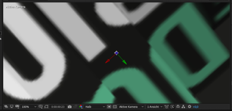
\includegraphics[width=2cm]{../img/logo_animation/2/screenshot_logo_5.PNG} }}
\qquad
 \subfloat[Screenshot: Animation 6]{{
\includegraphics[width=2cm]{../img/logo_animation/2/screenshot_logo_6.PNG} }}
\qquad
 \subfloat[Screenshot: Animation 7]{{
\includegraphics[width=2cm]{../img/logo_animation/2/screenshot_logo_7.PNG} }}
\caption{Screenshots Animations 2}%
 \label{fig:Screenshots Animations 2}%
\end{figure}

Im Anschluss wurde ein CC Light Sweep Effekt hinzugefügt und dafür gesorgt, dass das Logo kurz glänzt. Mit der Bestimmung der Richtung verläuft dieser Effekt von links oben nach rechts unten. Dieser Effekt ist auf der Abbildung \ref{fig:Screenshots Animations 3} zu sehen.

\begin{figure}[h]
\centering
 \subfloat[Screenshot: Animation 8]{{
\includegraphics[width=2cm]{../img/logo_animation/3/screenshot_logo_8.PNG} }}
\qquad
 \subfloat[Screenshot: Animation 9]{{
\includegraphics[width=2cm]{../img/logo_animation/3/screenshot_logo_9.PNG} }}
\qquad
 \subfloat[Screenshot: Animation 10]{{
\includegraphics[width=2cm]{../img/logo_animation/3/screenshot_logo_10.PNG} }}
\caption{Screenshots Animations 3}%
 \label{fig:Screenshots Animations 3}%
\end{figure}

\subsubsection{Produktion Video Intro}
Für einen Einstieg in die Geschichtsthematik des Spieles wurde der Betrachter mittels einer Kamerafahrt über das Meer an den eigentlichen Veranstaltungsort mitgenommen.
Dafür wurde ein längliches Bild angefertigt, das in AfterEffects zu einer Komposition hinzugefügt wurde. Anschließend wurde eine neue “Kamera” erstellt und die 3D-Funktionen der Kompositionsebene aktiviert. Nun mussten nur noch zwei Keyframes gewählt werden, den Startkeyframe am unteren, sowie den Endkeyframe am oberen Ende des Bildes.
Da Wasser, noch spezifischer gesehen Wellenbewegungen, sehr komplex zu animieren sind, wurde für die nächste Szene eine Wellenreihe in Adobe Animate angefertigt. Das Programm ermöglichte es die “Meereszacken” durch Anfertigung und Abspielen verschiedenster Frames zum Rotieren zu bringen. In After Effects importiert ergaben diese hintereinander liegenden Reihen in unterschiedlicher Ablaufgeschwindigkeit die Illusion einer sich bewegenden Meeresoberfläche. 
Das angefertigte Schiff musste jetzt an die Bewegungen der vordersten Welle angepasst werden. Diese Bildverschiebung kann in After Effects durch das Verändern der Position als auch Rotation sowie durch das Setzen mehrerer Keyframes (siehe Abbildung x) visualisiert werden. Auch der Hintergrund sowie der Blitz musste vorerst angefertigt und implementiert werden. Um das Aufleuchten des Blitzes naturgetreuer darzustellen, wurde seine Darstellung zwischen Erscheinen und Verschwinden noch verdoppelt. 

\begin{figure}
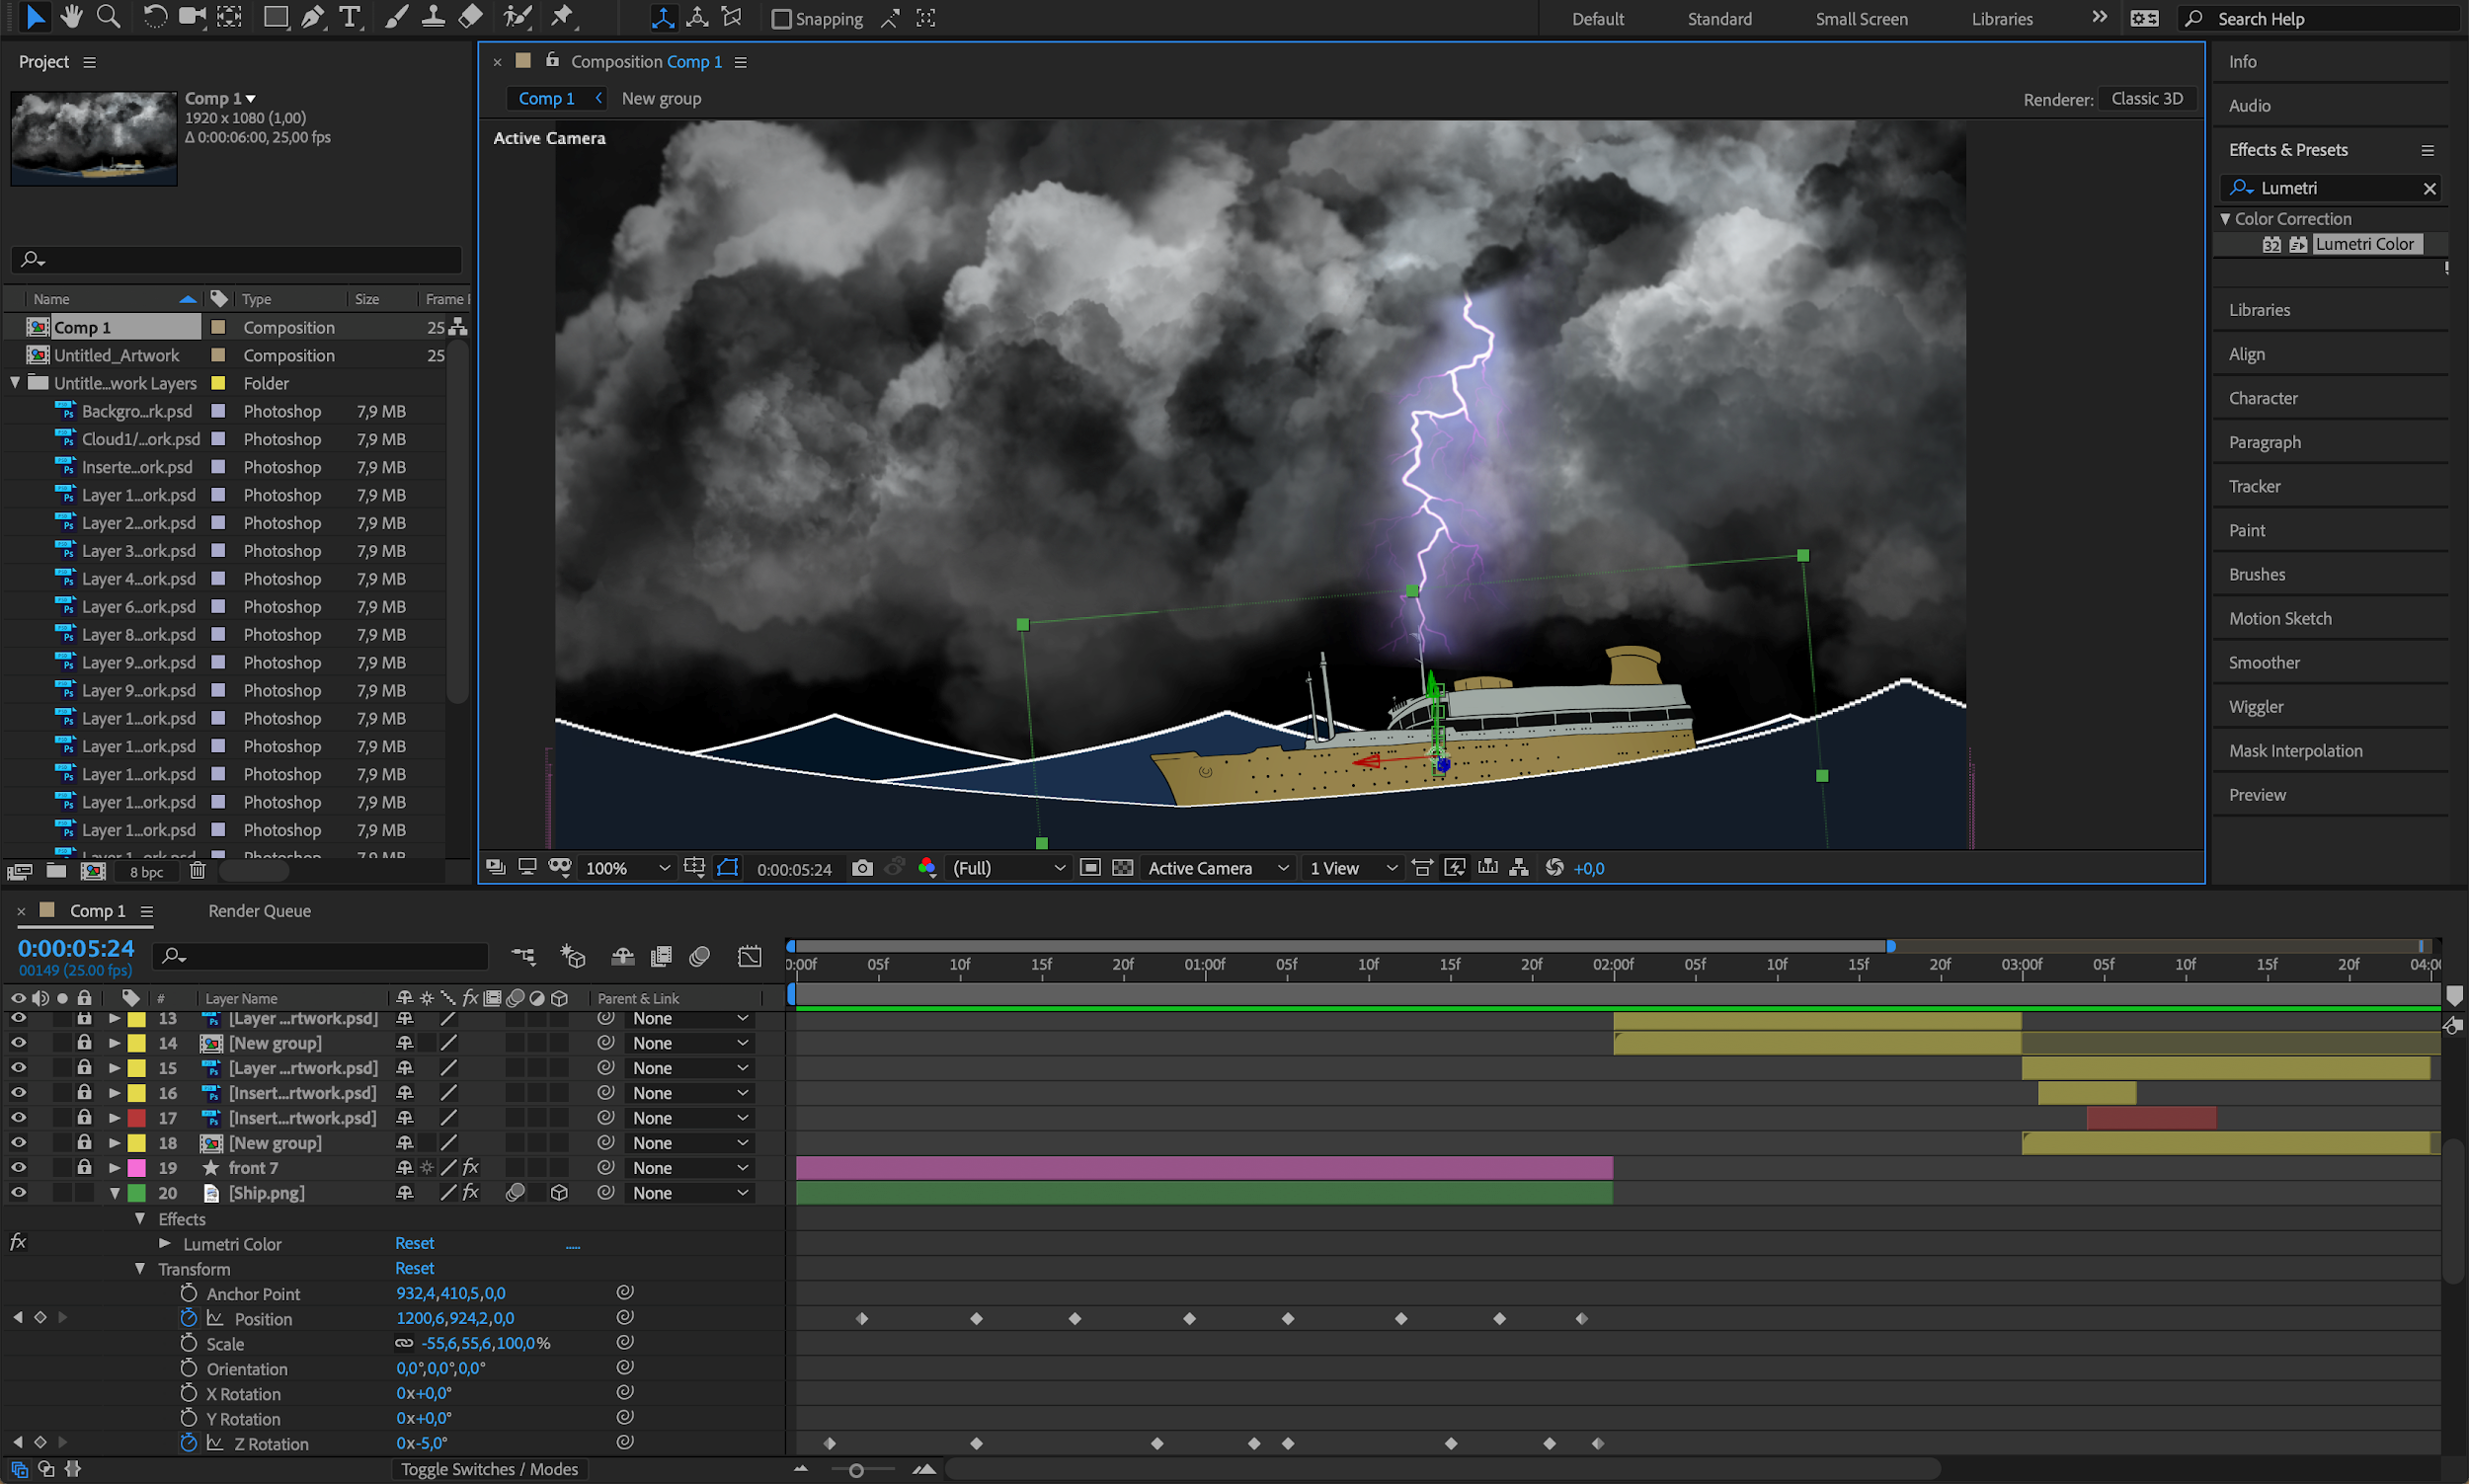
\includegraphics[width=0.5\textwidth]{../img/screenshot_aftereffects_intro.PNG}
\caption{Screenshot: After Effects Intro}
\label{fig:Screenshot: After Effects Intro}
\end{figure}